% Graphic for TeX using PGF
% Title: /tmp/UML.dia
% Creator: Dia v0.97.3
% CreationDate: Sun May  9 12:42:43 2021
% For: ivanfm
% \usepackage{tikz}
% The following commands are not supported in PSTricks at present
% We define them conditionally, so when they are implemented,
% this pgf file will use them.
\ifx\du\undefined
  \newlength{\du}
\fi
\setlength{\du}{15\unitlength}
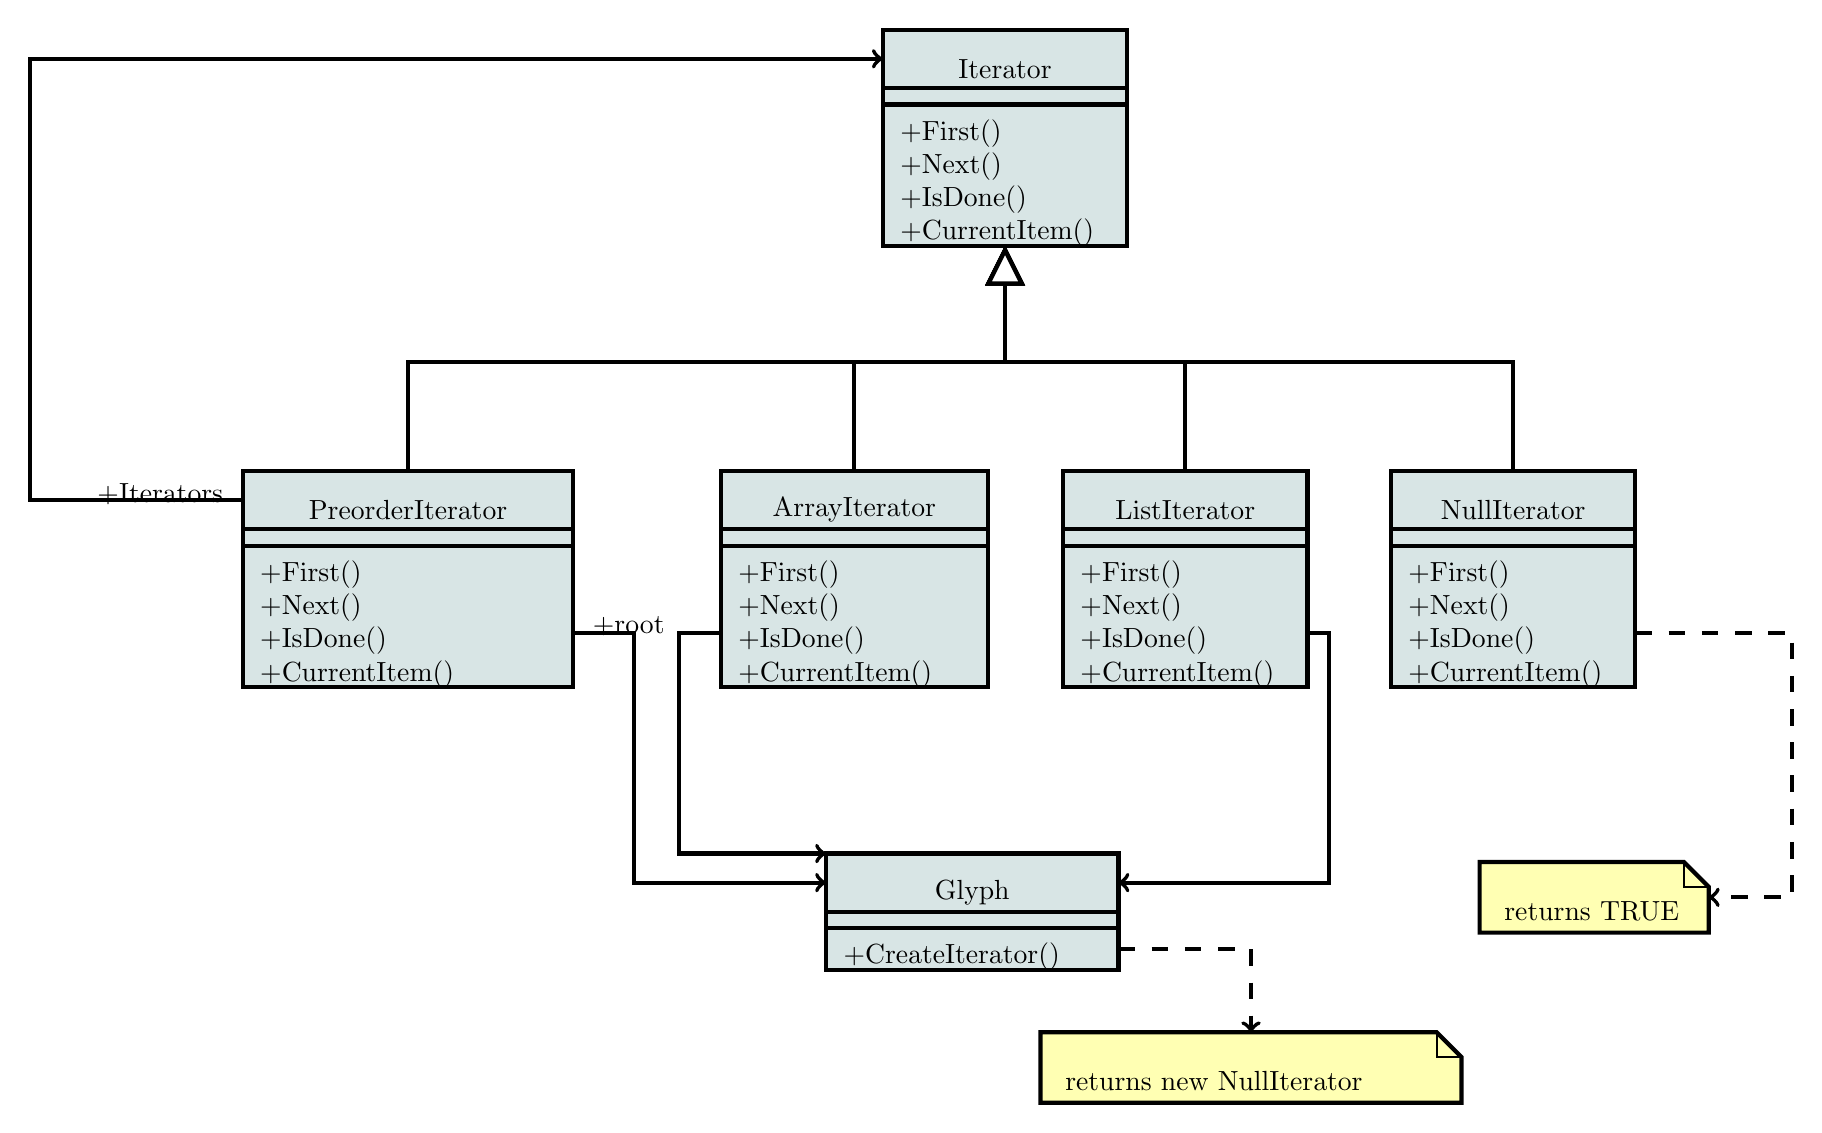
\begin{tikzpicture}
\pgftransformxscale{1.000000}
\pgftransformyscale{-1.000000}
\definecolor{dialinecolor}{rgb}{0.000000, 0.000000, 0.000000}
\pgfsetstrokecolor{dialinecolor}
\definecolor{dialinecolor}{rgb}{1.000000, 1.000000, 1.000000}
\pgfsetfillcolor{dialinecolor}
\pgfsetlinewidth{0.100000\du}
\pgfsetdash{}{0pt}
\pgfsetmiterjoin
\pgfsetbuttcap
{
\definecolor{dialinecolor}{rgb}{0.000000, 0.000000, 0.000000}
\pgfsetfillcolor{dialinecolor}
% was here!!!
\pgfsetarrowsend{to}
\definecolor{dialinecolor}{rgb}{0.000000, 0.000000, 0.000000}
\pgfsetstrokecolor{dialinecolor}
\draw (5.880000\du,12.530000\du)--(0.750000\du,12.530000\du)--(0.750000\du,1.900000\du)--(21.300000\du,1.900000\du);
}
% setfont left to latex
\definecolor{dialinecolor}{rgb}{0.000000, 0.000000, 0.000000}
\pgfsetstrokecolor{dialinecolor}
\node[anchor=west] at (0.850000\du,7.064072\du){};
\definecolor{dialinecolor}{rgb}{0.000000, 0.000000, 0.000000}
\pgfsetstrokecolor{dialinecolor}
\node[anchor=east] at (5.680000\du,12.379072\du){+Iterators};
\definecolor{dialinecolor}{rgb}{0.000000, 0.000000, 0.000000}
\pgfsetstrokecolor{dialinecolor}
\node[anchor=east] at (5.680000\du,13.179072\du){};
\definecolor{dialinecolor}{rgb}{0.000000, 0.000000, 0.000000}
\pgfsetstrokecolor{dialinecolor}
\node[anchor=east] at (20.300000\du,1.749072\du){};
\pgfsetlinewidth{0.100000\du}
\pgfsetdash{}{0pt}
\pgfsetmiterjoin
\pgfsetbuttcap
{
\definecolor{dialinecolor}{rgb}{0.000000, 0.000000, 0.000000}
\pgfsetfillcolor{dialinecolor}
% was here!!!
\definecolor{dialinecolor}{rgb}{0.000000, 0.000000, 0.000000}
\pgfsetstrokecolor{dialinecolor}
\draw (24.245000\du,6.400000\du)--(24.245000\du,9.200000\du)--(9.862500\du,9.200000\du)--(9.862500\du,11.830000\du);
}
\definecolor{dialinecolor}{rgb}{0.000000, 0.000000, 0.000000}
\pgfsetstrokecolor{dialinecolor}
\draw (24.245000\du,7.311803\du)--(24.245000\du,9.200000\du)--(9.862500\du,9.200000\du)--(9.862500\du,11.830000\du);
\pgfsetmiterjoin
\definecolor{dialinecolor}{rgb}{1.000000, 1.000000, 1.000000}
\pgfsetfillcolor{dialinecolor}
\fill (24.645000\du,7.311803\du)--(24.245000\du,6.511803\du)--(23.845000\du,7.311803\du)--cycle;
\pgfsetlinewidth{0.100000\du}
\pgfsetdash{}{0pt}
\pgfsetmiterjoin
\definecolor{dialinecolor}{rgb}{0.000000, 0.000000, 0.000000}
\pgfsetstrokecolor{dialinecolor}
\draw (24.645000\du,7.311803\du)--(24.245000\du,6.511803\du)--(23.845000\du,7.311803\du)--cycle;
% setfont left to latex
\pgfsetlinewidth{0.100000\du}
\pgfsetdash{}{0pt}
\definecolor{dialinecolor}{rgb}{0.847059, 0.898039, 0.898039}
\pgfsetfillcolor{dialinecolor}
\fill (19.931900\du,21.045400\du)--(19.931900\du,22.445400\du)--(26.976900\du,22.445400\du)--(26.976900\du,21.045400\du)--cycle;
\definecolor{dialinecolor}{rgb}{0.000000, 0.000000, 0.000000}
\pgfsetstrokecolor{dialinecolor}
\draw (19.931900\du,21.045400\du)--(19.931900\du,22.445400\du)--(26.976900\du,22.445400\du)--(26.976900\du,21.045400\du)--cycle;
% setfont left to latex
\definecolor{dialinecolor}{rgb}{0.000000, 0.000000, 0.000000}
\pgfsetstrokecolor{dialinecolor}
\node at (23.454400\du,21.987978\du){Glyph};
\definecolor{dialinecolor}{rgb}{0.847059, 0.898039, 0.898039}
\pgfsetfillcolor{dialinecolor}
\fill (19.931900\du,22.445400\du)--(19.931900\du,22.845400\du)--(26.976900\du,22.845400\du)--(26.976900\du,22.445400\du)--cycle;
\definecolor{dialinecolor}{rgb}{0.000000, 0.000000, 0.000000}
\pgfsetstrokecolor{dialinecolor}
\draw (19.931900\du,22.445400\du)--(19.931900\du,22.845400\du)--(26.976900\du,22.845400\du)--(26.976900\du,22.445400\du)--cycle;
\definecolor{dialinecolor}{rgb}{0.847059, 0.898039, 0.898039}
\pgfsetfillcolor{dialinecolor}
\fill (19.931900\du,22.845400\du)--(19.931900\du,23.845400\du)--(26.976900\du,23.845400\du)--(26.976900\du,22.845400\du)--cycle;
\definecolor{dialinecolor}{rgb}{0.000000, 0.000000, 0.000000}
\pgfsetstrokecolor{dialinecolor}
\draw (19.931900\du,22.845400\du)--(19.931900\du,23.845400\du)--(26.976900\du,23.845400\du)--(26.976900\du,22.845400\du)--cycle;
% setfont left to latex
\definecolor{dialinecolor}{rgb}{0.000000, 0.000000, 0.000000}
\pgfsetstrokecolor{dialinecolor}
\node[anchor=west] at (20.081900\du,23.539462\du){+CreateIterator()};
\pgfsetlinewidth{0.100000\du}
\pgfsetdash{}{0pt}
\pgfsetmiterjoin
\pgfsetbuttcap
{
\definecolor{dialinecolor}{rgb}{0.000000, 0.000000, 0.000000}
\pgfsetfillcolor{dialinecolor}
% was here!!!
\definecolor{dialinecolor}{rgb}{0.000000, 0.000000, 0.000000}
\pgfsetstrokecolor{dialinecolor}
\draw (24.245000\du,6.400000\du)--(24.245000\du,9.200000\du)--(20.615000\du,9.200000\du)--(20.615000\du,11.830000\du);
}
\definecolor{dialinecolor}{rgb}{0.000000, 0.000000, 0.000000}
\pgfsetstrokecolor{dialinecolor}
\draw (24.245000\du,7.311803\du)--(24.245000\du,9.200000\du)--(20.615000\du,9.200000\du)--(20.615000\du,11.830000\du);
\pgfsetmiterjoin
\definecolor{dialinecolor}{rgb}{1.000000, 1.000000, 1.000000}
\pgfsetfillcolor{dialinecolor}
\fill (24.645000\du,7.311803\du)--(24.245000\du,6.511803\du)--(23.845000\du,7.311803\du)--cycle;
\pgfsetlinewidth{0.100000\du}
\pgfsetdash{}{0pt}
\pgfsetmiterjoin
\definecolor{dialinecolor}{rgb}{0.000000, 0.000000, 0.000000}
\pgfsetstrokecolor{dialinecolor}
\draw (24.645000\du,7.311803\du)--(24.245000\du,6.511803\du)--(23.845000\du,7.311803\du)--cycle;
% setfont left to latex
\pgfsetlinewidth{0.100000\du}
\pgfsetdash{}{0pt}
\pgfsetmiterjoin
\pgfsetbuttcap
{
\definecolor{dialinecolor}{rgb}{0.000000, 0.000000, 0.000000}
\pgfsetfillcolor{dialinecolor}
% was here!!!
\definecolor{dialinecolor}{rgb}{0.000000, 0.000000, 0.000000}
\pgfsetstrokecolor{dialinecolor}
\draw (24.245000\du,6.400000\du)--(24.245000\du,9.200000\du)--(28.585000\du,9.200000\du)--(28.585000\du,11.830000\du);
}
\definecolor{dialinecolor}{rgb}{0.000000, 0.000000, 0.000000}
\pgfsetstrokecolor{dialinecolor}
\draw (24.245000\du,7.311803\du)--(24.245000\du,9.200000\du)--(28.585000\du,9.200000\du)--(28.585000\du,11.830000\du);
\pgfsetmiterjoin
\definecolor{dialinecolor}{rgb}{1.000000, 1.000000, 1.000000}
\pgfsetfillcolor{dialinecolor}
\fill (24.645000\du,7.311803\du)--(24.245000\du,6.511803\du)--(23.845000\du,7.311803\du)--cycle;
\pgfsetlinewidth{0.100000\du}
\pgfsetdash{}{0pt}
\pgfsetmiterjoin
\definecolor{dialinecolor}{rgb}{0.000000, 0.000000, 0.000000}
\pgfsetstrokecolor{dialinecolor}
\draw (24.645000\du,7.311803\du)--(24.245000\du,6.511803\du)--(23.845000\du,7.311803\du)--cycle;
% setfont left to latex
\pgfsetlinewidth{0.100000\du}
\pgfsetdash{}{0pt}
\pgfsetmiterjoin
\pgfsetbuttcap
{
\definecolor{dialinecolor}{rgb}{0.000000, 0.000000, 0.000000}
\pgfsetfillcolor{dialinecolor}
% was here!!!
\definecolor{dialinecolor}{rgb}{0.000000, 0.000000, 0.000000}
\pgfsetstrokecolor{dialinecolor}
\draw (24.245000\du,6.400000\du)--(24.245000\du,9.200000\du)--(36.485000\du,9.200000\du)--(36.485000\du,11.830000\du);
}
\definecolor{dialinecolor}{rgb}{0.000000, 0.000000, 0.000000}
\pgfsetstrokecolor{dialinecolor}
\draw (24.245000\du,7.311803\du)--(24.245000\du,9.200000\du)--(36.485000\du,9.200000\du)--(36.485000\du,11.830000\du);
\pgfsetmiterjoin
\definecolor{dialinecolor}{rgb}{1.000000, 1.000000, 1.000000}
\pgfsetfillcolor{dialinecolor}
\fill (24.645000\du,7.311803\du)--(24.245000\du,6.511803\du)--(23.845000\du,7.311803\du)--cycle;
\pgfsetlinewidth{0.100000\du}
\pgfsetdash{}{0pt}
\pgfsetmiterjoin
\definecolor{dialinecolor}{rgb}{0.000000, 0.000000, 0.000000}
\pgfsetstrokecolor{dialinecolor}
\draw (24.645000\du,7.311803\du)--(24.245000\du,6.511803\du)--(23.845000\du,7.311803\du)--cycle;
% setfont left to latex
\pgfsetlinewidth{0.100000\du}
\pgfsetdash{}{0pt}
\pgfsetmiterjoin
\pgfsetbuttcap
{
\definecolor{dialinecolor}{rgb}{0.000000, 0.000000, 0.000000}
\pgfsetfillcolor{dialinecolor}
% was here!!!
\pgfsetarrowsend{to}
\definecolor{dialinecolor}{rgb}{0.000000, 0.000000, 0.000000}
\pgfsetstrokecolor{dialinecolor}
\draw (13.845000\du,15.730000\du)--(15.300000\du,15.730000\du)--(15.300000\du,21.745400\du)--(19.931900\du,21.745400\du);
}
% setfont left to latex
\definecolor{dialinecolor}{rgb}{0.000000, 0.000000, 0.000000}
\pgfsetstrokecolor{dialinecolor}
\node[anchor=west] at (15.400000\du,18.586772\du){};
\definecolor{dialinecolor}{rgb}{0.000000, 0.000000, 0.000000}
\pgfsetstrokecolor{dialinecolor}
\node[anchor=west] at (14.045000\du,15.579072\du){+root};
\definecolor{dialinecolor}{rgb}{0.000000, 0.000000, 0.000000}
\pgfsetstrokecolor{dialinecolor}
\node[anchor=west] at (14.045000\du,16.379072\du){};
\definecolor{dialinecolor}{rgb}{0.000000, 0.000000, 0.000000}
\pgfsetstrokecolor{dialinecolor}
\node[anchor=east] at (18.931900\du,21.594472\du){};
\pgfsetlinewidth{0.100000\du}
\pgfsetdash{}{0pt}
\pgfsetmiterjoin
\pgfsetbuttcap
{
\definecolor{dialinecolor}{rgb}{0.000000, 0.000000, 0.000000}
\pgfsetfillcolor{dialinecolor}
% was here!!!
\pgfsetarrowsend{to}
\definecolor{dialinecolor}{rgb}{0.000000, 0.000000, 0.000000}
\pgfsetstrokecolor{dialinecolor}
\draw (17.398700\du,15.730000\du)--(16.398700\du,15.730000\du)--(16.398700\du,21.045400\du)--(19.931900\du,21.045400\du);
}
% setfont left to latex
\definecolor{dialinecolor}{rgb}{0.000000, 0.000000, 0.000000}
\pgfsetstrokecolor{dialinecolor}
\node[anchor=west] at (16.498700\du,18.236772\du){};
\definecolor{dialinecolor}{rgb}{0.000000, 0.000000, 0.000000}
\pgfsetstrokecolor{dialinecolor}
\node[anchor=east] at (17.198700\du,15.579072\du){};
\definecolor{dialinecolor}{rgb}{0.000000, 0.000000, 0.000000}
\pgfsetstrokecolor{dialinecolor}
\node[anchor=east] at (18.931900\du,20.894472\du){};
\pgfsetlinewidth{0.100000\du}
\pgfsetdash{}{0pt}
\pgfsetmiterjoin
\pgfsetbuttcap
{
\definecolor{dialinecolor}{rgb}{0.000000, 0.000000, 0.000000}
\pgfsetfillcolor{dialinecolor}
% was here!!!
\pgfsetarrowsend{to}
\definecolor{dialinecolor}{rgb}{0.000000, 0.000000, 0.000000}
\pgfsetstrokecolor{dialinecolor}
\draw (31.530000\du,15.730000\du)--(32.040000\du,15.730000\du)--(32.040000\du,21.745400\du)--(26.976900\du,21.745400\du);
}
% setfont left to latex
\definecolor{dialinecolor}{rgb}{0.000000, 0.000000, 0.000000}
\pgfsetstrokecolor{dialinecolor}
\node[anchor=west] at (32.140000\du,18.586772\du){};
\definecolor{dialinecolor}{rgb}{0.000000, 0.000000, 0.000000}
\pgfsetstrokecolor{dialinecolor}
\node[anchor=west] at (31.730000\du,15.579072\du){};
\definecolor{dialinecolor}{rgb}{0.000000, 0.000000, 0.000000}
\pgfsetstrokecolor{dialinecolor}
\node[anchor=west] at (27.976900\du,21.594472\du){};
\pgfsetlinewidth{0.100000\du}
\pgfsetdash{}{0pt}
\definecolor{dialinecolor}{rgb}{1.000000, 1.000000, 0.701961}
\pgfsetfillcolor{dialinecolor}
\fill (25.100000\du,25.350000\du)--(34.640000\du,25.350000\du)--(35.240000\du,25.950000\du)--(35.240000\du,27.050000\du)--(25.100000\du,27.050000\du)--cycle;
\definecolor{dialinecolor}{rgb}{0.000000, 0.000000, 0.000000}
\pgfsetstrokecolor{dialinecolor}
\draw (25.100000\du,25.350000\du)--(34.640000\du,25.350000\du)--(35.240000\du,25.950000\du)--(35.240000\du,27.050000\du)--(25.100000\du,27.050000\du)--cycle;
\pgfsetlinewidth{0.050000\du}
\definecolor{dialinecolor}{rgb}{0.000000, 0.000000, 0.000000}
\pgfsetstrokecolor{dialinecolor}
\draw (34.640000\du,25.350000\du)--(34.640000\du,25.950000\du)--(35.240000\du,25.950000\du);
% setfont left to latex
\definecolor{dialinecolor}{rgb}{0.000000, 0.000000, 0.000000}
\pgfsetstrokecolor{dialinecolor}
\node[anchor=west] at (25.450000\du,26.532813\du){returns new NullIterator};
\pgfsetlinewidth{0.100000\du}
\pgfsetdash{{1.000000\du}{1.000000\du}}{0\du}
\pgfsetdash{{0.400000\du}{0.400000\du}}{0\du}
\pgfsetmiterjoin
\pgfsetbuttcap
{
\definecolor{dialinecolor}{rgb}{0.000000, 0.000000, 0.000000}
\pgfsetfillcolor{dialinecolor}
% was here!!!
\pgfsetarrowsend{to}
\definecolor{dialinecolor}{rgb}{0.000000, 0.000000, 0.000000}
\pgfsetstrokecolor{dialinecolor}
\draw (26.976900\du,23.345400\du)--(30.170000\du,23.345400\du)--(30.170000\du,25.350000\du);
}
% setfont left to latex
\pgfsetlinewidth{0.100000\du}
\pgfsetdash{}{0pt}
\definecolor{dialinecolor}{rgb}{1.000000, 1.000000, 0.701961}
\pgfsetfillcolor{dialinecolor}
\fill (35.677300\du,21.250000\du)--(40.597300\du,21.250000\du)--(41.197300\du,21.850000\du)--(41.197300\du,22.950000\du)--(35.677300\du,22.950000\du)--cycle;
\definecolor{dialinecolor}{rgb}{0.000000, 0.000000, 0.000000}
\pgfsetstrokecolor{dialinecolor}
\draw (35.677300\du,21.250000\du)--(40.597300\du,21.250000\du)--(41.197300\du,21.850000\du)--(41.197300\du,22.950000\du)--(35.677300\du,22.950000\du)--cycle;
\pgfsetlinewidth{0.050000\du}
\definecolor{dialinecolor}{rgb}{0.000000, 0.000000, 0.000000}
\pgfsetstrokecolor{dialinecolor}
\draw (40.597300\du,21.250000\du)--(40.597300\du,21.850000\du)--(41.197300\du,21.850000\du);
% setfont left to latex
\definecolor{dialinecolor}{rgb}{0.000000, 0.000000, 0.000000}
\pgfsetstrokecolor{dialinecolor}
\node[anchor=west] at (36.027300\du,22.432813\du){returns TRUE};
\pgfsetlinewidth{0.100000\du}
\pgfsetdash{{0.400000\du}{0.400000\du}}{0\du}
\pgfsetdash{{0.400000\du}{0.400000\du}}{0\du}
\pgfsetmiterjoin
\pgfsetbuttcap
{
\definecolor{dialinecolor}{rgb}{0.000000, 0.000000, 0.000000}
\pgfsetfillcolor{dialinecolor}
% was here!!!
\pgfsetarrowsend{to}
\definecolor{dialinecolor}{rgb}{0.000000, 0.000000, 0.000000}
\pgfsetstrokecolor{dialinecolor}
\draw (39.430000\du,15.730000\du)--(43.195200\du,15.730000\du)--(43.195200\du,22.100000\du)--(41.197300\du,22.100000\du);
}
% setfont left to latex
\pgfsetlinewidth{0.100000\du}
\pgfsetdash{}{0pt}
\definecolor{dialinecolor}{rgb}{0.847059, 0.898039, 0.898039}
\pgfsetfillcolor{dialinecolor}
\fill (21.300000\du,1.200000\du)--(21.300000\du,2.600000\du)--(27.190000\du,2.600000\du)--(27.190000\du,1.200000\du)--cycle;
\definecolor{dialinecolor}{rgb}{0.000000, 0.000000, 0.000000}
\pgfsetstrokecolor{dialinecolor}
\draw (21.300000\du,1.200000\du)--(21.300000\du,2.600000\du)--(27.190000\du,2.600000\du)--(27.190000\du,1.200000\du)--cycle;
% setfont left to latex
\definecolor{dialinecolor}{rgb}{0.000000, 0.000000, 0.000000}
\pgfsetstrokecolor{dialinecolor}
\node at (24.245000\du,2.142578\du){Iterator};
\definecolor{dialinecolor}{rgb}{0.847059, 0.898039, 0.898039}
\pgfsetfillcolor{dialinecolor}
\fill (21.300000\du,2.600000\du)--(21.300000\du,3.000000\du)--(27.190000\du,3.000000\du)--(27.190000\du,2.600000\du)--cycle;
\definecolor{dialinecolor}{rgb}{0.000000, 0.000000, 0.000000}
\pgfsetstrokecolor{dialinecolor}
\draw (21.300000\du,2.600000\du)--(21.300000\du,3.000000\du)--(27.190000\du,3.000000\du)--(27.190000\du,2.600000\du)--cycle;
\definecolor{dialinecolor}{rgb}{0.847059, 0.898039, 0.898039}
\pgfsetfillcolor{dialinecolor}
\fill (21.300000\du,3.000000\du)--(21.300000\du,6.400000\du)--(27.190000\du,6.400000\du)--(27.190000\du,3.000000\du)--cycle;
\definecolor{dialinecolor}{rgb}{0.000000, 0.000000, 0.000000}
\pgfsetstrokecolor{dialinecolor}
\draw (21.300000\du,3.000000\du)--(21.300000\du,6.400000\du)--(27.190000\du,6.400000\du)--(27.190000\du,3.000000\du)--cycle;
% setfont left to latex
\definecolor{dialinecolor}{rgb}{0.000000, 0.000000, 0.000000}
\pgfsetstrokecolor{dialinecolor}
\node[anchor=west] at (21.450000\du,3.694062\du){+First()};
% setfont left to latex
\definecolor{dialinecolor}{rgb}{0.000000, 0.000000, 0.000000}
\pgfsetstrokecolor{dialinecolor}
\node[anchor=west] at (21.450000\du,4.494063\du){+Next()};
% setfont left to latex
\definecolor{dialinecolor}{rgb}{0.000000, 0.000000, 0.000000}
\pgfsetstrokecolor{dialinecolor}
\node[anchor=west] at (21.450000\du,5.294062\du){+IsDone()};
% setfont left to latex
\definecolor{dialinecolor}{rgb}{0.000000, 0.000000, 0.000000}
\pgfsetstrokecolor{dialinecolor}
\node[anchor=west] at (21.450000\du,6.094062\du){+CurrentItem()};
\pgfsetlinewidth{0.100000\du}
\pgfsetdash{}{0pt}
\definecolor{dialinecolor}{rgb}{0.847059, 0.898039, 0.898039}
\pgfsetfillcolor{dialinecolor}
\fill (5.880000\du,11.830000\du)--(5.880000\du,13.230000\du)--(13.845000\du,13.230000\du)--(13.845000\du,11.830000\du)--cycle;
\definecolor{dialinecolor}{rgb}{0.000000, 0.000000, 0.000000}
\pgfsetstrokecolor{dialinecolor}
\draw (5.880000\du,11.830000\du)--(5.880000\du,13.230000\du)--(13.845000\du,13.230000\du)--(13.845000\du,11.830000\du)--cycle;
% setfont left to latex
\definecolor{dialinecolor}{rgb}{0.000000, 0.000000, 0.000000}
\pgfsetstrokecolor{dialinecolor}
\node at (9.862500\du,12.772578\du){PreorderIterator};
\definecolor{dialinecolor}{rgb}{0.847059, 0.898039, 0.898039}
\pgfsetfillcolor{dialinecolor}
\fill (5.880000\du,13.230000\du)--(5.880000\du,13.630000\du)--(13.845000\du,13.630000\du)--(13.845000\du,13.230000\du)--cycle;
\definecolor{dialinecolor}{rgb}{0.000000, 0.000000, 0.000000}
\pgfsetstrokecolor{dialinecolor}
\draw (5.880000\du,13.230000\du)--(5.880000\du,13.630000\du)--(13.845000\du,13.630000\du)--(13.845000\du,13.230000\du)--cycle;
\definecolor{dialinecolor}{rgb}{0.847059, 0.898039, 0.898039}
\pgfsetfillcolor{dialinecolor}
\fill (5.880000\du,13.630000\du)--(5.880000\du,17.030000\du)--(13.845000\du,17.030000\du)--(13.845000\du,13.630000\du)--cycle;
\definecolor{dialinecolor}{rgb}{0.000000, 0.000000, 0.000000}
\pgfsetstrokecolor{dialinecolor}
\draw (5.880000\du,13.630000\du)--(5.880000\du,17.030000\du)--(13.845000\du,17.030000\du)--(13.845000\du,13.630000\du)--cycle;
% setfont left to latex
\definecolor{dialinecolor}{rgb}{0.000000, 0.000000, 0.000000}
\pgfsetstrokecolor{dialinecolor}
\node[anchor=west] at (6.030000\du,14.324063\du){+First()};
% setfont left to latex
\definecolor{dialinecolor}{rgb}{0.000000, 0.000000, 0.000000}
\pgfsetstrokecolor{dialinecolor}
\node[anchor=west] at (6.030000\du,15.124062\du){+Next()};
% setfont left to latex
\definecolor{dialinecolor}{rgb}{0.000000, 0.000000, 0.000000}
\pgfsetstrokecolor{dialinecolor}
\node[anchor=west] at (6.030000\du,15.924062\du){+IsDone()};
% setfont left to latex
\definecolor{dialinecolor}{rgb}{0.000000, 0.000000, 0.000000}
\pgfsetstrokecolor{dialinecolor}
\node[anchor=west] at (6.030000\du,16.724062\du){+CurrentItem()};
\pgfsetlinewidth{0.100000\du}
\pgfsetdash{}{0pt}
\definecolor{dialinecolor}{rgb}{0.847059, 0.898039, 0.898039}
\pgfsetfillcolor{dialinecolor}
\fill (17.398700\du,11.830000\du)--(17.398700\du,13.230000\du)--(23.831200\du,13.230000\du)--(23.831200\du,11.830000\du)--cycle;
\definecolor{dialinecolor}{rgb}{0.000000, 0.000000, 0.000000}
\pgfsetstrokecolor{dialinecolor}
\draw (17.398700\du,11.830000\du)--(17.398700\du,13.230000\du)--(23.831200\du,13.230000\du)--(23.831200\du,11.830000\du)--cycle;
% setfont left to latex
\definecolor{dialinecolor}{rgb}{0.000000, 0.000000, 0.000000}
\pgfsetstrokecolor{dialinecolor}
\node at (20.614950\du,12.772578\du){ArrayIterator};
\definecolor{dialinecolor}{rgb}{0.847059, 0.898039, 0.898039}
\pgfsetfillcolor{dialinecolor}
\fill (17.398700\du,13.230000\du)--(17.398700\du,13.630000\du)--(23.831200\du,13.630000\du)--(23.831200\du,13.230000\du)--cycle;
\definecolor{dialinecolor}{rgb}{0.000000, 0.000000, 0.000000}
\pgfsetstrokecolor{dialinecolor}
\draw (17.398700\du,13.230000\du)--(17.398700\du,13.630000\du)--(23.831200\du,13.630000\du)--(23.831200\du,13.230000\du)--cycle;
\definecolor{dialinecolor}{rgb}{0.847059, 0.898039, 0.898039}
\pgfsetfillcolor{dialinecolor}
\fill (17.398700\du,13.630000\du)--(17.398700\du,17.030000\du)--(23.831200\du,17.030000\du)--(23.831200\du,13.630000\du)--cycle;
\definecolor{dialinecolor}{rgb}{0.000000, 0.000000, 0.000000}
\pgfsetstrokecolor{dialinecolor}
\draw (17.398700\du,13.630000\du)--(17.398700\du,17.030000\du)--(23.831200\du,17.030000\du)--(23.831200\du,13.630000\du)--cycle;
% setfont left to latex
\definecolor{dialinecolor}{rgb}{0.000000, 0.000000, 0.000000}
\pgfsetstrokecolor{dialinecolor}
\node[anchor=west] at (17.548700\du,14.324063\du){+First()};
% setfont left to latex
\definecolor{dialinecolor}{rgb}{0.000000, 0.000000, 0.000000}
\pgfsetstrokecolor{dialinecolor}
\node[anchor=west] at (17.548700\du,15.124062\du){+Next()};
% setfont left to latex
\definecolor{dialinecolor}{rgb}{0.000000, 0.000000, 0.000000}
\pgfsetstrokecolor{dialinecolor}
\node[anchor=west] at (17.548700\du,15.924062\du){+IsDone()};
% setfont left to latex
\definecolor{dialinecolor}{rgb}{0.000000, 0.000000, 0.000000}
\pgfsetstrokecolor{dialinecolor}
\node[anchor=west] at (17.548700\du,16.724062\du){+CurrentItem()};
\pgfsetlinewidth{0.100000\du}
\pgfsetdash{}{0pt}
\definecolor{dialinecolor}{rgb}{0.847059, 0.898039, 0.898039}
\pgfsetfillcolor{dialinecolor}
\fill (33.540000\du,11.830000\du)--(33.540000\du,13.230000\du)--(39.430000\du,13.230000\du)--(39.430000\du,11.830000\du)--cycle;
\definecolor{dialinecolor}{rgb}{0.000000, 0.000000, 0.000000}
\pgfsetstrokecolor{dialinecolor}
\draw (33.540000\du,11.830000\du)--(33.540000\du,13.230000\du)--(39.430000\du,13.230000\du)--(39.430000\du,11.830000\du)--cycle;
% setfont left to latex
\definecolor{dialinecolor}{rgb}{0.000000, 0.000000, 0.000000}
\pgfsetstrokecolor{dialinecolor}
\node at (36.485000\du,12.772578\du){NullIterator};
\definecolor{dialinecolor}{rgb}{0.847059, 0.898039, 0.898039}
\pgfsetfillcolor{dialinecolor}
\fill (33.540000\du,13.230000\du)--(33.540000\du,13.630000\du)--(39.430000\du,13.630000\du)--(39.430000\du,13.230000\du)--cycle;
\definecolor{dialinecolor}{rgb}{0.000000, 0.000000, 0.000000}
\pgfsetstrokecolor{dialinecolor}
\draw (33.540000\du,13.230000\du)--(33.540000\du,13.630000\du)--(39.430000\du,13.630000\du)--(39.430000\du,13.230000\du)--cycle;
\definecolor{dialinecolor}{rgb}{0.847059, 0.898039, 0.898039}
\pgfsetfillcolor{dialinecolor}
\fill (33.540000\du,13.630000\du)--(33.540000\du,17.030000\du)--(39.430000\du,17.030000\du)--(39.430000\du,13.630000\du)--cycle;
\definecolor{dialinecolor}{rgb}{0.000000, 0.000000, 0.000000}
\pgfsetstrokecolor{dialinecolor}
\draw (33.540000\du,13.630000\du)--(33.540000\du,17.030000\du)--(39.430000\du,17.030000\du)--(39.430000\du,13.630000\du)--cycle;
% setfont left to latex
\definecolor{dialinecolor}{rgb}{0.000000, 0.000000, 0.000000}
\pgfsetstrokecolor{dialinecolor}
\node[anchor=west] at (33.690000\du,14.324063\du){+First()};
% setfont left to latex
\definecolor{dialinecolor}{rgb}{0.000000, 0.000000, 0.000000}
\pgfsetstrokecolor{dialinecolor}
\node[anchor=west] at (33.690000\du,15.124062\du){+Next()};
% setfont left to latex
\definecolor{dialinecolor}{rgb}{0.000000, 0.000000, 0.000000}
\pgfsetstrokecolor{dialinecolor}
\node[anchor=west] at (33.690000\du,15.924062\du){+IsDone()};
% setfont left to latex
\definecolor{dialinecolor}{rgb}{0.000000, 0.000000, 0.000000}
\pgfsetstrokecolor{dialinecolor}
\node[anchor=west] at (33.690000\du,16.724062\du){+CurrentItem()};
\pgfsetlinewidth{0.100000\du}
\pgfsetdash{}{0pt}
\definecolor{dialinecolor}{rgb}{0.847059, 0.898039, 0.898039}
\pgfsetfillcolor{dialinecolor}
\fill (25.640000\du,11.830000\du)--(25.640000\du,13.230000\du)--(31.530000\du,13.230000\du)--(31.530000\du,11.830000\du)--cycle;
\definecolor{dialinecolor}{rgb}{0.000000, 0.000000, 0.000000}
\pgfsetstrokecolor{dialinecolor}
\draw (25.640000\du,11.830000\du)--(25.640000\du,13.230000\du)--(31.530000\du,13.230000\du)--(31.530000\du,11.830000\du)--cycle;
% setfont left to latex
\definecolor{dialinecolor}{rgb}{0.000000, 0.000000, 0.000000}
\pgfsetstrokecolor{dialinecolor}
\node at (28.585000\du,12.772578\du){ListIterator};
\definecolor{dialinecolor}{rgb}{0.847059, 0.898039, 0.898039}
\pgfsetfillcolor{dialinecolor}
\fill (25.640000\du,13.230000\du)--(25.640000\du,13.630000\du)--(31.530000\du,13.630000\du)--(31.530000\du,13.230000\du)--cycle;
\definecolor{dialinecolor}{rgb}{0.000000, 0.000000, 0.000000}
\pgfsetstrokecolor{dialinecolor}
\draw (25.640000\du,13.230000\du)--(25.640000\du,13.630000\du)--(31.530000\du,13.630000\du)--(31.530000\du,13.230000\du)--cycle;
\definecolor{dialinecolor}{rgb}{0.847059, 0.898039, 0.898039}
\pgfsetfillcolor{dialinecolor}
\fill (25.640000\du,13.630000\du)--(25.640000\du,17.030000\du)--(31.530000\du,17.030000\du)--(31.530000\du,13.630000\du)--cycle;
\definecolor{dialinecolor}{rgb}{0.000000, 0.000000, 0.000000}
\pgfsetstrokecolor{dialinecolor}
\draw (25.640000\du,13.630000\du)--(25.640000\du,17.030000\du)--(31.530000\du,17.030000\du)--(31.530000\du,13.630000\du)--cycle;
% setfont left to latex
\definecolor{dialinecolor}{rgb}{0.000000, 0.000000, 0.000000}
\pgfsetstrokecolor{dialinecolor}
\node[anchor=west] at (25.790000\du,14.324063\du){+First()};
% setfont left to latex
\definecolor{dialinecolor}{rgb}{0.000000, 0.000000, 0.000000}
\pgfsetstrokecolor{dialinecolor}
\node[anchor=west] at (25.790000\du,15.124062\du){+Next()};
% setfont left to latex
\definecolor{dialinecolor}{rgb}{0.000000, 0.000000, 0.000000}
\pgfsetstrokecolor{dialinecolor}
\node[anchor=west] at (25.790000\du,15.924062\du){+IsDone()};
% setfont left to latex
\definecolor{dialinecolor}{rgb}{0.000000, 0.000000, 0.000000}
\pgfsetstrokecolor{dialinecolor}
\node[anchor=west] at (25.790000\du,16.724062\du){+CurrentItem()};
\end{tikzpicture}
